\chapter{Modelo de lattice-Boltzmann}
\graphicspath{{figs/cap3/}}
\label{cap3}

\section{LBM Multifásicos}

En éste capítulo se presentara cuál es el modelo de LB para la resolución de problemas de transferencia de calor con flujos multifásicos y cambio de fase.

Generalmente es difícil resolver las ecuaciones de la mecánica de los fluidos. Las soluciones analíticas de los problemas que pueden ser halladas son escasas, como el caso de flujos \textit{Couette} o \textit{Poisueuille}. Problemas que contengan una geometría más compleja u otras condiciones de contorno; poseen una gran dificultad para encontrar la solución de las ecuaciones de la mecánica de fluidos, si es que el problema la posee. Debido a ello las soluciónes se obtienen numéricamente \cite{kruger2017lattice}(sec 3.1). Es de importancia el desarrollo de métodos numéricos que resuelvan los problemas de forma paralela para así reducir el tiempo de cálculo.

Debido a que los problemas que se plantean resolver en el presente trabajo es de transferencia de calor en flujos multifásicos con cambio de fase, la escala de del fluido que se decide adoptar es la mesoscópica. Considerando la escala y siendo un problema multifásico, se opta por resolver numéricamente mediante LBM. 

Los LBM multifásicos tienen la particularidad de que la frontera entre las fases no son resueltas con exactitud. Dicha interfaz es representada de forma difusa con un cierto tamaño en la grilla, siendo una importante ventaja para el cálculo puesto que la interfaz no debe ser encontrada.\cite{parrill2019reviews}.

Los modelos para resolver los flujos multifásicos son tres : \textit{color gradient}, \textit{Shan Chen model} o \textit{pseudopotential} y \textit{Free-energy}. 

\begin{itemize}
	
	\item \textit{Color gradient} fue el primer modelo de LBE para flujos multifásicos siendo desarrollado por Gunstensen \cite{gunstensen1991lattice}. Las fases y las interacciones entre las partículas son denotadas mediante diferentes colores. Por medio del modelado local del gradiente de color que se encuentra asociado a la diferencia de las densidades de las dos fases, se conoce como es la segregación y separación de las fases.
	
	\item \textit{Shan Chen model} o \textit{pseudopotential} surge del modelo de colores donde la redistribución de las particulas de fluido está basada en \textit{color gradient}. La fuerza de interacción proviene de la diferencia entre las fuerzas promedio del modelo molecular  entre ambos lados de la interfaz. Shan and Chen \cite{shan1993lattice} presentaron un modelo de LBE (referenciado como modelo SC) que podría representar la interacción entre partículas fluidas de forma más precisa y directa introduciendo un pseudo potencial. 
	
	\item \textit{Free-energy} es un modelo un tipo alternativo de LBE desarrollado por Swift \cite{swift1995lattice} para modelos multifásicos/multicomponentes basado en la teoría de energía libre (\textit{free-energy}). Debido a que la fenomenología representada en los modelos de LBE de color y pseudo potenciales son la misma. La idea básica del nuevo método es realizar una función de distribución de equilibrio basada en funciones de energía libre, en las cuales se incorpora el tensor de presión termodinámico.\cite{guo2013lattice}(sec 7) .
	
\end{itemize}


\section{Modelo pseudopotencial}

El modelo pseudopotencial es el adoptado en el presente trabajo para abordar los problemas descriptos en \ref{cap2}.


La obtención de la ecuación de lattice-Boltzmann (LBE) a través de la ecuación de Boltzmann se encuentra descripta en \cite{kruger2017lattice} (sec 3.4 y 3.5 ). Primero se explica la discretización en el espacio de velocidades, en el segundo la del espacio físico, temporal e integración de las características.


Para entender el LBM, hay que saber que el mismo deriva de discretizar la ecuación de Boltzmann en los espacios de velocidad, físico y temporal.  


Un LBM es el \textit{DdQq} (\textit{d} - dimensional , \textit{q} velocidades). La figura \ref{fig:D1Q3_D2Q9} muestra como es el conjunto de velocidades del modelo D1Q3 y D2Q9.

En el presente trabajo el LBM es $D2Q9$. 

\begin{figure}[h]
	\centering
    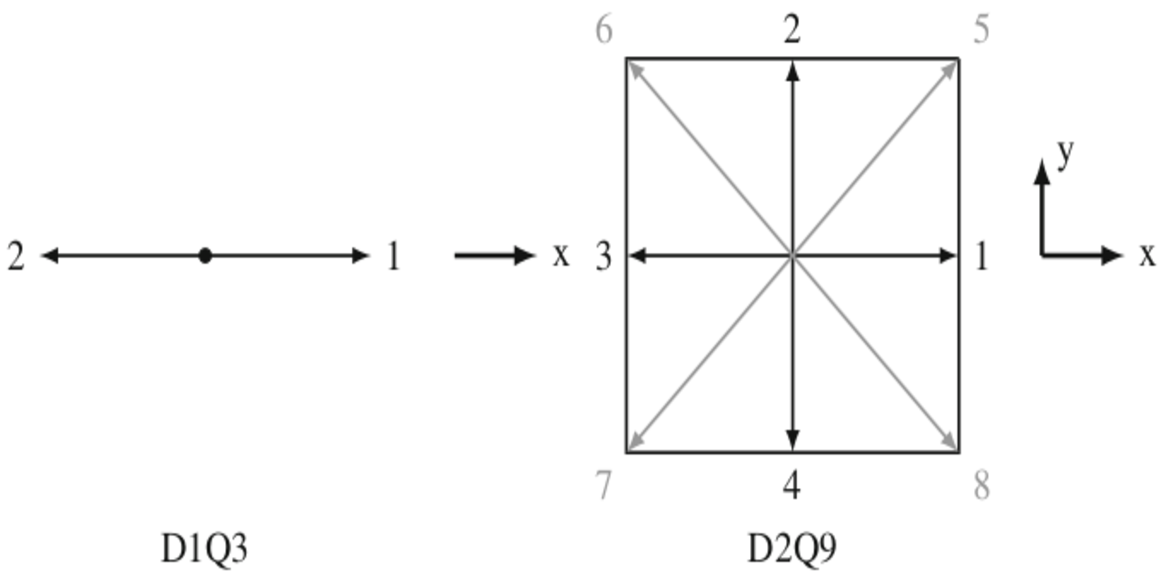
\includegraphics[width=.8\textwidth]{figs/cap3/D1Q3_D2Q9}
	\caption{Conjunto de velocidades de los modelos D1Q3 y D2Q9. \cite{kruger2017lattice}}
	\label{fig:D1Q3_D2Q9}	
\end{figure}

El problema físico a resolver cuenta con una región, la cuál se le realizará un mallado para discretizar el espacio. El nodo i - ésimo de la malla posee las coordenadas ${\bar{X}}_{i} = (x,y,z)$, a su vez densidad $\rho_{i}$ y temperatura $T_{i}$. La velocidad en el nodo tiene las componentes ${\bar{U}}_{i} = ({U}_{ix},{U}_{iy},{U}_{iz})$. El espacio de velocidades indica como es la propagación de las propiedades en la grilla. Dicha velocidad de grilla $\mathbf{e}_{i}$ posee $\alpha$ componentes donde $\alpha = q $. 

Para el modelo D2Q9 la figura \ref{fig:D1Q3_D2Q9} muestra un esquema de las velocidades de grilla del nodo i - ésimo y la Ec. (\ref{eq:velgrilla}) el valor adoptado.


\begin{equation}
    {\mathbf{e}}_{i} =  
    \left( \begin{array}{c} 
                e_{i0} \\ e_{i1}\\ e_{i2}\\ e_{i3}\\ e_{i4}\\ e_{i5}\\
                e_{i6}\\ e_{i7}\\ e_{i8}\\
            \end{array}
    \right) =
    \left( \begin{array}{c} 
        (0,0,0) \\ (1,0,0) \\ (0,1,0) \\(-1,0,0) \\ (0,-1,0) \\ (1,1,0) \\
        (-1,1,0) \\ (-1,-1,0) \\ (1,-1,0)\\ 
    \end{array}
    \right) 
    \label{eq:velgrilla}
\end{equation}

A su vez cada uno de los nodos de la grilla posee un campo de distribución $f_{i}$ también con $\alpha$ componentes. Mediante el campo se puede obtener las variables macroscópicas del problema.

Para el desarrollo de la solución de los problemas que se describieron en \ref{cap2}, se utiliza el modelo pseudopotencial de dos ecuaciones con operador MRT, siendo desarrollado por Fogliatto \cite{fogliatto2018modelado} y \colorbox{green}{citar eq energia}


\section{Modelo pseudopotencial de dos ecuaciones con operador MRT}

\subsection{Ecuación hidrodinámica}


La resolución de las ecuaciones hidrodinámicas pueden analizarse mediante la evolución de una función de distribución dada por \cite{li2013lattice}: 	

\begin{equation}
    \mathbf{f}(\mathbf{x} + \mathbf{e} \> \delta_{t} , t + \delta_{t}) = \mathbf{M}^{-1} \left[ \mathbf{m} - \mathbf{\Lambda}(\mathbf{m} - \mathbf{m}^{(eq)}) + \delta_{t} \left( \mathbf{I} - 0,5 \mathbf{\Lambda} \right) \mathbf{\bar{S}}  \right]_{(\mathbf{x},t)} 
    \label{eq:fieldmom}
\end{equation}

donde $\textit{f}_{\alpha}$ es la distribución de densidad en el espacio de poblaciones, t el tiempo, $\mathbf{x}$ la posición espacial, \textit{\textbf{e}} las velocidades discretas a lo largo de la direcciones $\alpha$ y $\delta_{t}$ el paso de tiempo. En este caso, la notación usada en la Ec. (\ref{eq:fieldmom}) implica que la compontente $\alpha-ésima$ del miembro izquierdo está dada por $f_{\alpha}(x + e_{\alpha} \delta_{t}  , t + \delta_{t} )$ . El miembro derecho de la Ec. (\ref{eq:fieldmom}) corresponde a la etapa de post-colisión definida en el espacio de momentos, donde \textbf{M} es una matriz de transformación ortogonal, $\mathbf{m} = \mathbf{M} \cdot \mathbf{f}$ , $\mathbf{m}_{eq} = \mathbf{M} \cdot \mathbf{f}_{eq}$ , \textbf{I} el tensor identidad y $\mathbf{\bar{S}} = \mathbf{M} \mathbf{S}$ el término de fuente. Para una grilla D2Q9, $ \Lambda$ es una matriz diagonal:
    
\begin{align}
    \mathbf{\Lambda}  = diag ( {\tau_{\rho }}^{-1},{\tau_{e}}^{-1},{\tau_{\zeta }}^{-1},{\tau_{j}}^{-1},{\tau_{q}}^{-1},{\tau_{j}}^{-1},{\tau_{q}}^{-1},{\tau_{\nu }}^{-1},{\tau_{\nu}}^{-1}) 
    \label{eq:lambda}
\end{align}

mientras que la distribución de equilibrio está dada por:
        

\begin{align}
    m_{eq} =  \rho  \left( 1, - 2 + 3 {|u|}^{2} , 1 - 3{|u|}^{2} , u_{x} , - u_{x} , u_{y} , - u_{y} , {u_{x}}^{2} - {u_{y}}^{2} , u_{x} u_{y} \right) 
    \label{eq:m}
\end{align}


donde la densidad y velocidad macroscópica se obtienen mediante:

\begin{equation}
        \rho = \sum_{\alpha} f_{\alpha}
\end{equation}

\begin{equation}
    \rho \> \mathbf{u} = \sum_{\alpha} {\mathbf{e}}_{\alpha} \> f_{\alpha} + 0,5 \> {\delta}{t} \> \mathbf{F}
\end{equation}

En este caso, $ {\mathbf{F}} = (F_{x} , F_{y} ) = {\mathbf{F}}_{b} + {\mathbf{F}}_{int} $ es la fuerza total, ${\mathbf{F}}_{b}$ la fuerza volumétrica y ${\mathbf{F}}_{int}$ representa la fuerza de interacción que actúa sobre el sistema a través de un potencial $\psi(x)$:
    
\begin{equation}
    {\mathbf{F}}_{int} = - G \> \psi(\mathbf{x}) \sum_{\alpha=1}^{N} w({|{\mathbf{e}}_{\alpha}|}^{2}) \> \psi (\mathbf{x} + {\mathbf{e}}_{\alpha} \> \delta_{t}) \> {\mathbf{e}}_{\alpha} 
    \label{eq:fint}
\end{equation}

En la Ec. \ref{eq:fint}, G corresponde a la intensidad de interacción, $w({|{\mathbf{e}}_{\alpha}|}^{2})$ son los pesos correspondientes a una grilla D2Q9 y $\psi$ está dado por:

\begin{equation} 
    \psi(\rho) = \sqrt{\frac{2 (p_{EOS} - \rho {c_{s}}^{2})}{G {c}^{2}}}
\end{equation}

En el presente trabajo se adopta una EOS de VdW:

\begin{equation}
    \rho_{EOS} = \frac{\rho r t}{1- \rho B} - A {\rho}^{2}
\end{equation}

donde \textit{a} y \textit{b} son parámetros que determinan los valores críticos de temperatura, presión y densidad, y fueron fijados en $\textit{a} = 1$ y $\textit{b} = 4$. Finalmente, la fuerza de interacción se incorpora en la etapa de colisión mediante un término de fuente apropiado:

\begin{equation}
    \bar{S} = 
    \left[ \begin{array}{c} 
        0\\
        6 \mathbf{u}\cdot \mathbf{F} + \frac{12 \sigma {|{\mathbf{F}_{int}|}}^{2} }{{\psi}^{2} \delta_{t} (\tau_{e} - 0,5)}\\
        6 \mathbf{u}\cdot \mathbf{F} - \frac{12 \sigma {|{\mathbf{F}_{int}|}}^{2} }{{\psi}^{2} \delta_{t} (\tau_{\zeta } - 0,5)}\\
        F_{x}\\
        -F_{x}\\
        F_{y}\\
        -F_{y}\\
        2(u_{x} F_{x} - u_{y} F_{y} )\\
        (u_{x} F_{x} + u_{y} F_{y} )\\              
    \end{array}
    \right]    
\end{equation}

donde $\sigma$ es un parámetro libre que es utilizado para ajustar el problema de inconsistencia termodinámica, es decir, la diferencia entre las densidades de cada fase obtenidas en la simulación y aquellas determinadas por la EOS correspondiente.

\subsection{Ecuación energía}

Se debe acoplar una segunda ecuación LB para poder incorporar transferencia de calor al modelo de \cite{li2013lattice}. En particular, puede adoptarse una segunda distribución de poblaciones \textit{g} bajo un operador de colisión MRT:

\begin{equation}
    \mathbf{g^*}(\mathbf{x} + \mathbf{e} \delta_{t} ,t + \delta_{t}) = \mathbf{M}^{-1} \left[ \mathbf{n} - \mathbf{Q}(\mathbf{n} - \mathbf{n}^{(eq)}) + \delta_{t} \left( I - 0,5 Q \right) \hat{\Gamma}  \right]_{(\mathbf{x},t)}
    \label{eq:fieldenergy}
\end{equation}

donde $n = M g$ y $\hat{\Gamma}$es una fuente en el espacio de momentos. La temperatura macroscópica \textit{T} puede recuperarse mediante:

\begin{equation}
    T = \sum_{\alpha} g_{\alpha} + \frac{1}{2} \delta_{t} {\hat{\Gamma}}_{0}
\end{equation}

La matriz de coeficientes de relajación \textbf{Q} está compuesta por una parte diagonal

\begin{equation}
    \textit{diag} (Q) = {( q_{0} , q_{1} , q_{2} , q_{3} , q_{4} , q_{5} , q_{6} , q_{7} , q_{8} )}^{T}
\end{equation}

pero, a diferencia de $\lambda$ , presenta elementos extra diagonales no nulos dados por:

\begin{equation}
    Q_{3,4} = q_{4} \left( \frac{q_{3}}{2} - 1 \right)
\end{equation}

\begin{equation}
    Q_{5,6} = q_{6} \left( \frac{q_{5}}{2} - 1 \right)
\end{equation}

Si se define una distribución de equilibrio \textit{n} como:

\begin{equation}
    {\mathbf{n}}_{eq} = T { \left( 1, \alpha_{1}, \alpha_{2}, u_{x}, -u_{x}, u_{y}, -u_{y}, 0, 0 \right) }^{T}
\end{equation}

y el término fuente mediante:

\begin{equation}
    \hat{\Gamma} = {( s, 0, 0, 0, 0, 0, 0, 0, 0 )}^{T}
\end{equation}

con 

\begin{equation}
    s = \frac{\chi}{\rho} \bigtriangledown T \cdot \bigtriangledown \rho + T \left[ 1 - \frac{1}{\rho c_{\nu}} {\left( \frac{\delta p_{EOS}}{\delta T} \right)}_{\rho} \right] \bigtriangledown \cdot \mathbf{u}
\end{equation}

entonces la Ec. \ref{eq:fieldenergy} puede recuperar adecuadamente la ecuación macroscópica derivada por \cite{markus2011simulation}:

\begin{equation}
    \delta_{t} T + \bigtriangledown \cdot ( \mathbf{u} T ) = \chi {\bigtriangledown }^{2} T + s
\end{equation}

Por simplicidad, en este trabajo se considera una difusifidad térmica $\chi$ constante, la cual queda determinada mediante los factores de relajación de \textbf{Q} y los parámetros libres de ${\textbf{n}}_{eq}$ :

\begin{equation}
    \chi = \delta_{t} \left( \frac{1}{q_{3}} - \frac{1}{2} \right) \left( \frac{ 4 + 3 \alpha_{1} + 2 \alpha_{2}}{6} \right)
\end{equation}




%%% Local Variables: 
%%% mode: latex
%%% TeX-master: "template"
%%% End: 